\documentclass{beamer}	
\mode<presentation>
 
\usepackage{pdfpages}
\usepackage{fancyvrb}
\usepackage{chemarr}

\usepackage{amsmath}		%% mathematics typesetting
\usepackage{amssymb}
 
\usepackage{epigraph}   %% nice setting of quotations

\usepackage{tabularx} %% allows to use row colours in tables

\usepackage{ulem}

\usepackage{booktabs}

\usepackage{siunitx} %% tpyeset SI units

\usepackage{CJKutf8} %% typeset Chinese characters

\usepackage{pdfpages}%% include pdfs

\usepackage{subfigure}

\usepackage{animate} %% show animated gifs

\DeclareMathAlphabet{\mathcalligra}{T1}{calligra}{m}{n}

\newcommand{\heart}{\ensuremath\heartsuit} % make a heart if needed

% Color and Theme. Can be changed. However, this one's quite nice.
\usetheme{Madrid}
\definecolor{theme}{rgb}{0.84,0,0.21}
\usecolortheme[named=theme]{structure}


%%  Title information
\title[M14.1 Geschichte und Theorie]{M14.1 Historische Entwicklung und \\ Grundzüge der Wissenschaftstheorie}
\author[melanie.stefan@medicalschool-berlin.de]{M14 Wissenschaftliches Arbeiten}
\institute[]{Prof. Melanie Stefan - melanie.stefan@medicalschool-berlin.de}
\date{} 

% Table of contents to pop up at the beginning of each section
\AtBeginSection[]
{
  \begin{frame}<beamer>
    \frametitle{Outline}
    \tableofcontents[currentsection,currentsubsection]
  \end{frame}
}
 
\beamertemplatenavigationsymbolsempty

\begin{document}
 
  { \usebackgroundtemplate{\includegraphics[width=1.2\paperwidth]{MSB_Titelseite.pdf}} 
\begin{frame}

 \maketitle 

$\,$\\[6cm] 


\end{frame} 
}


%% Hook

\begin{frame}
\frametitle{Als Mediziner*in sollten Sie wissenschaftlich arbeiten können}

\begin{figure}
    \centering
    \subfigure{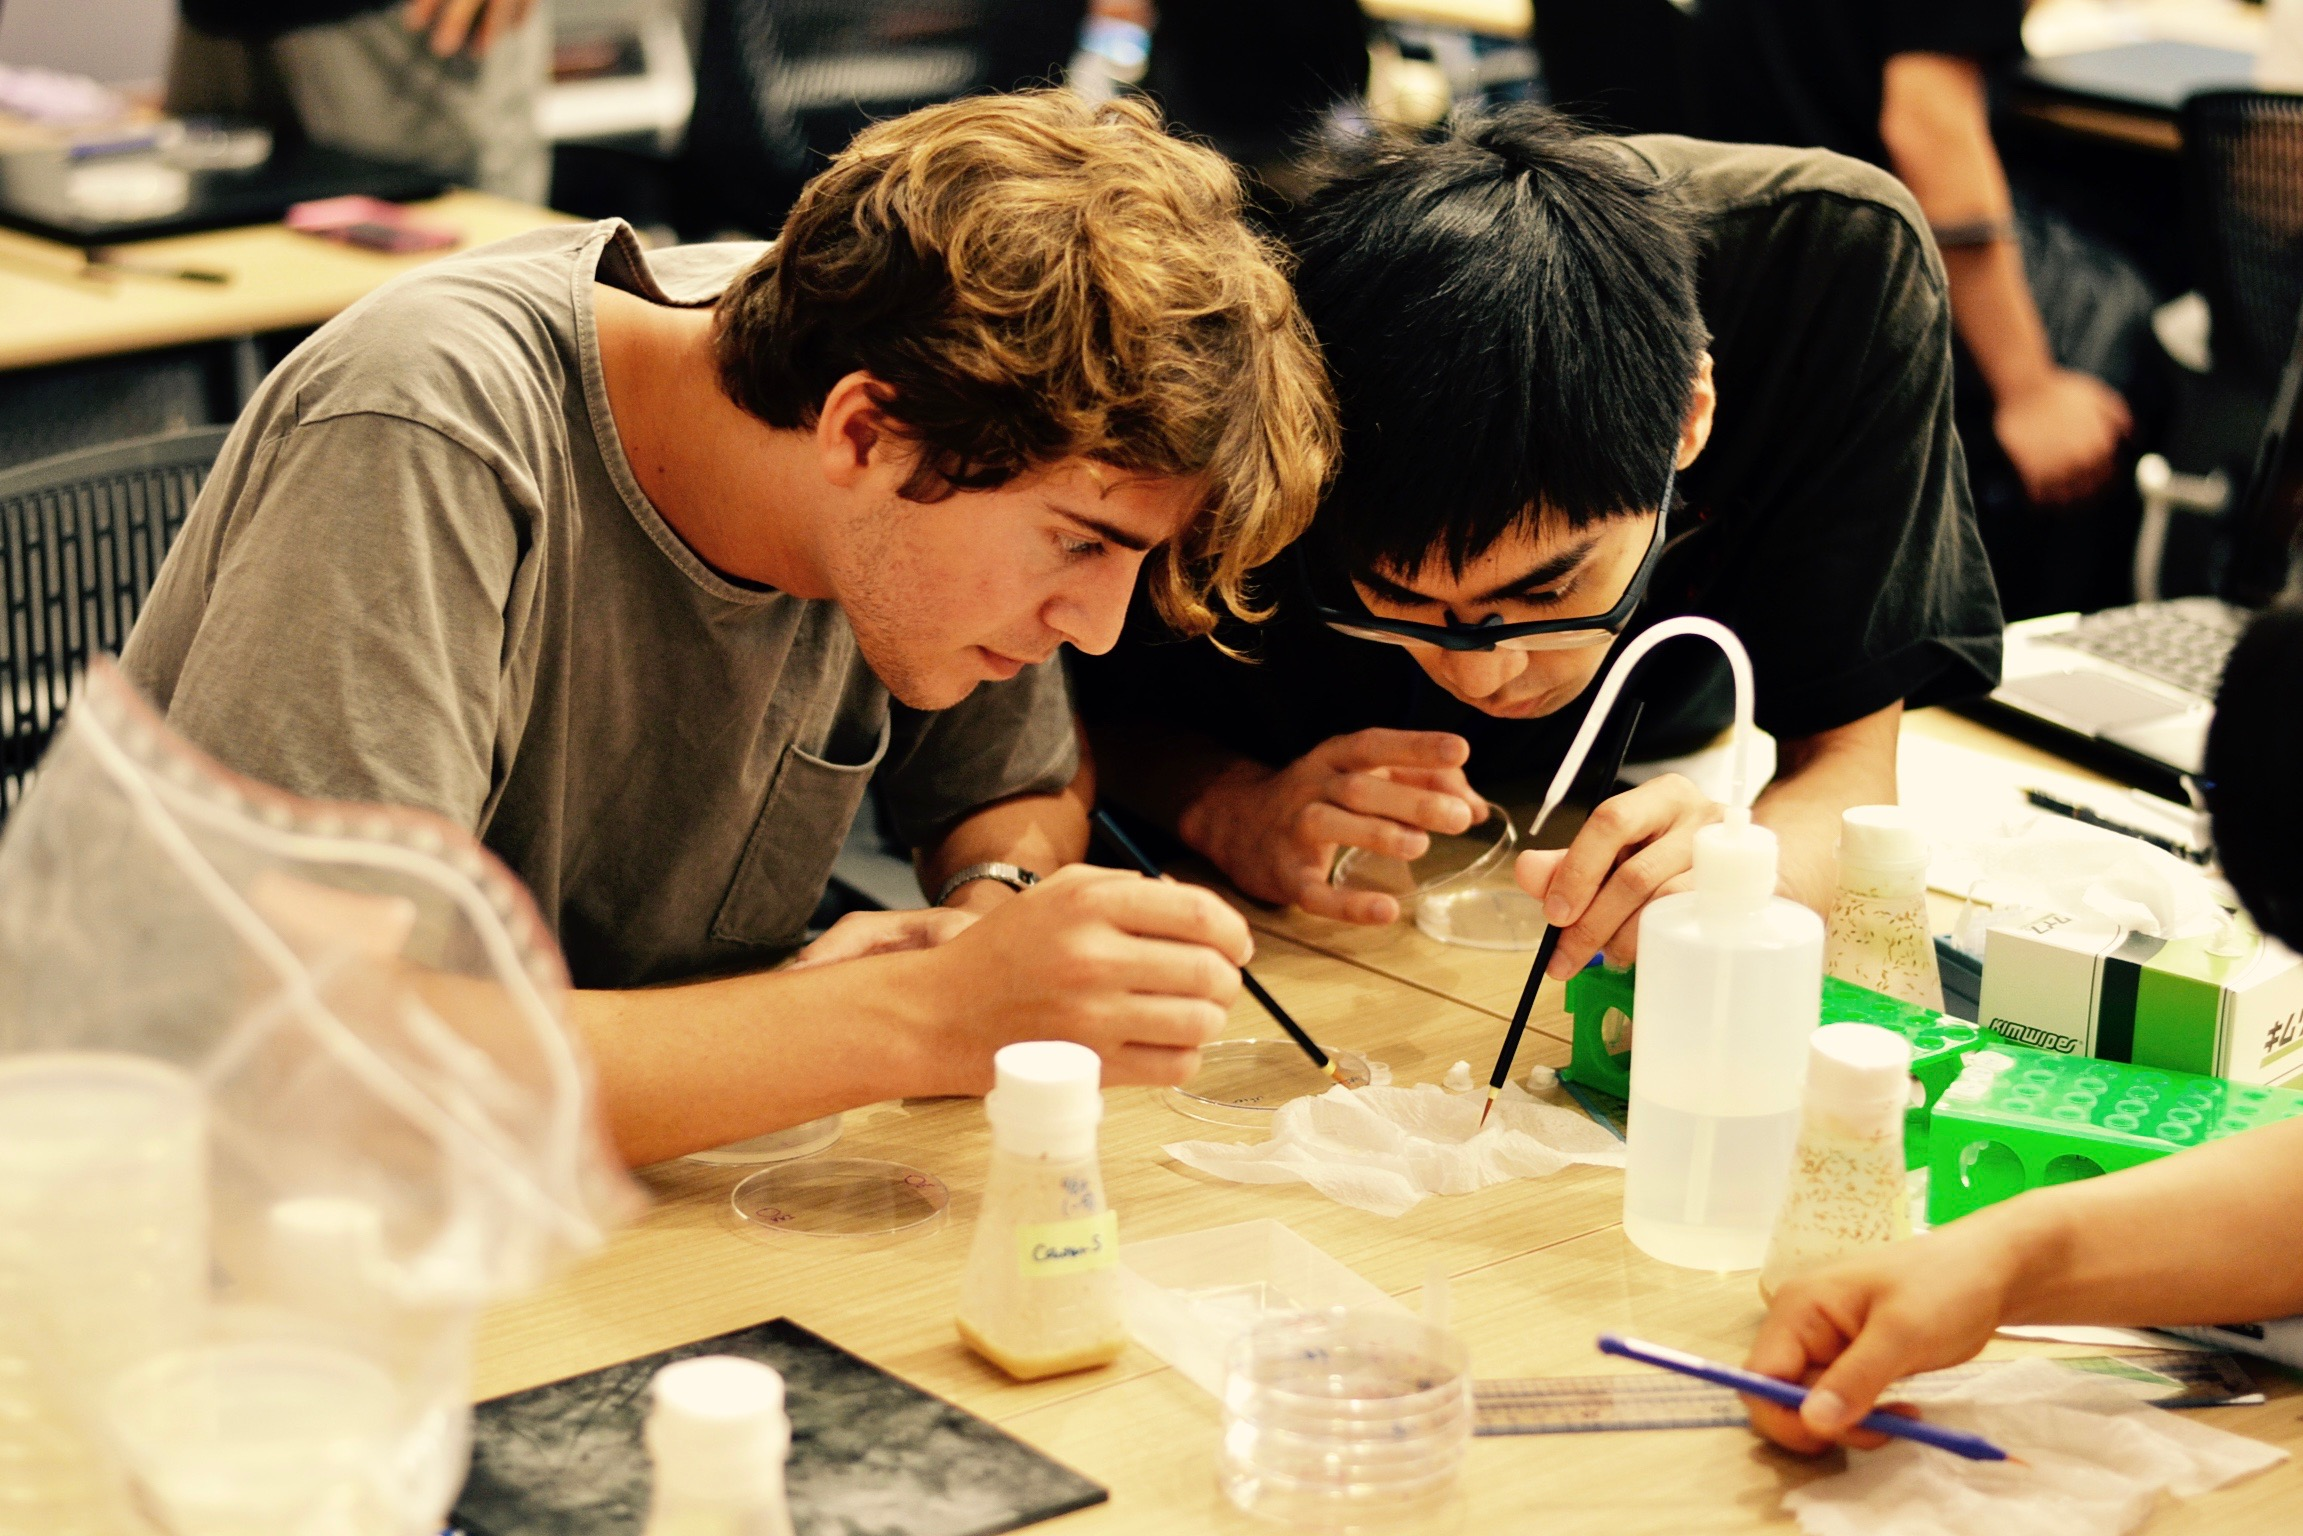
\includegraphics[width=0.4\textwidth]{collaborative_experiment.png}} 
    \subfigure{\includegraphics[width=0.4\textwidth]{presentations_audience.JPG}}\\
    
    \subfigure{\includegraphics[width=0.4\textwidth]{students_on_computers.jpg}}
    \subfigure{\includegraphics[width=0.4\textwidth]{student_presenting.jpg}}  
\end{figure}
\end{frame}

\begin{frame}
\frametitle{Als Mediziner*in sollten Sie wissenschaftlich arbeiten können - Aber wie? Und warum? Und was heißt das?}

\begin{figure}
    \centering
    \subfigure{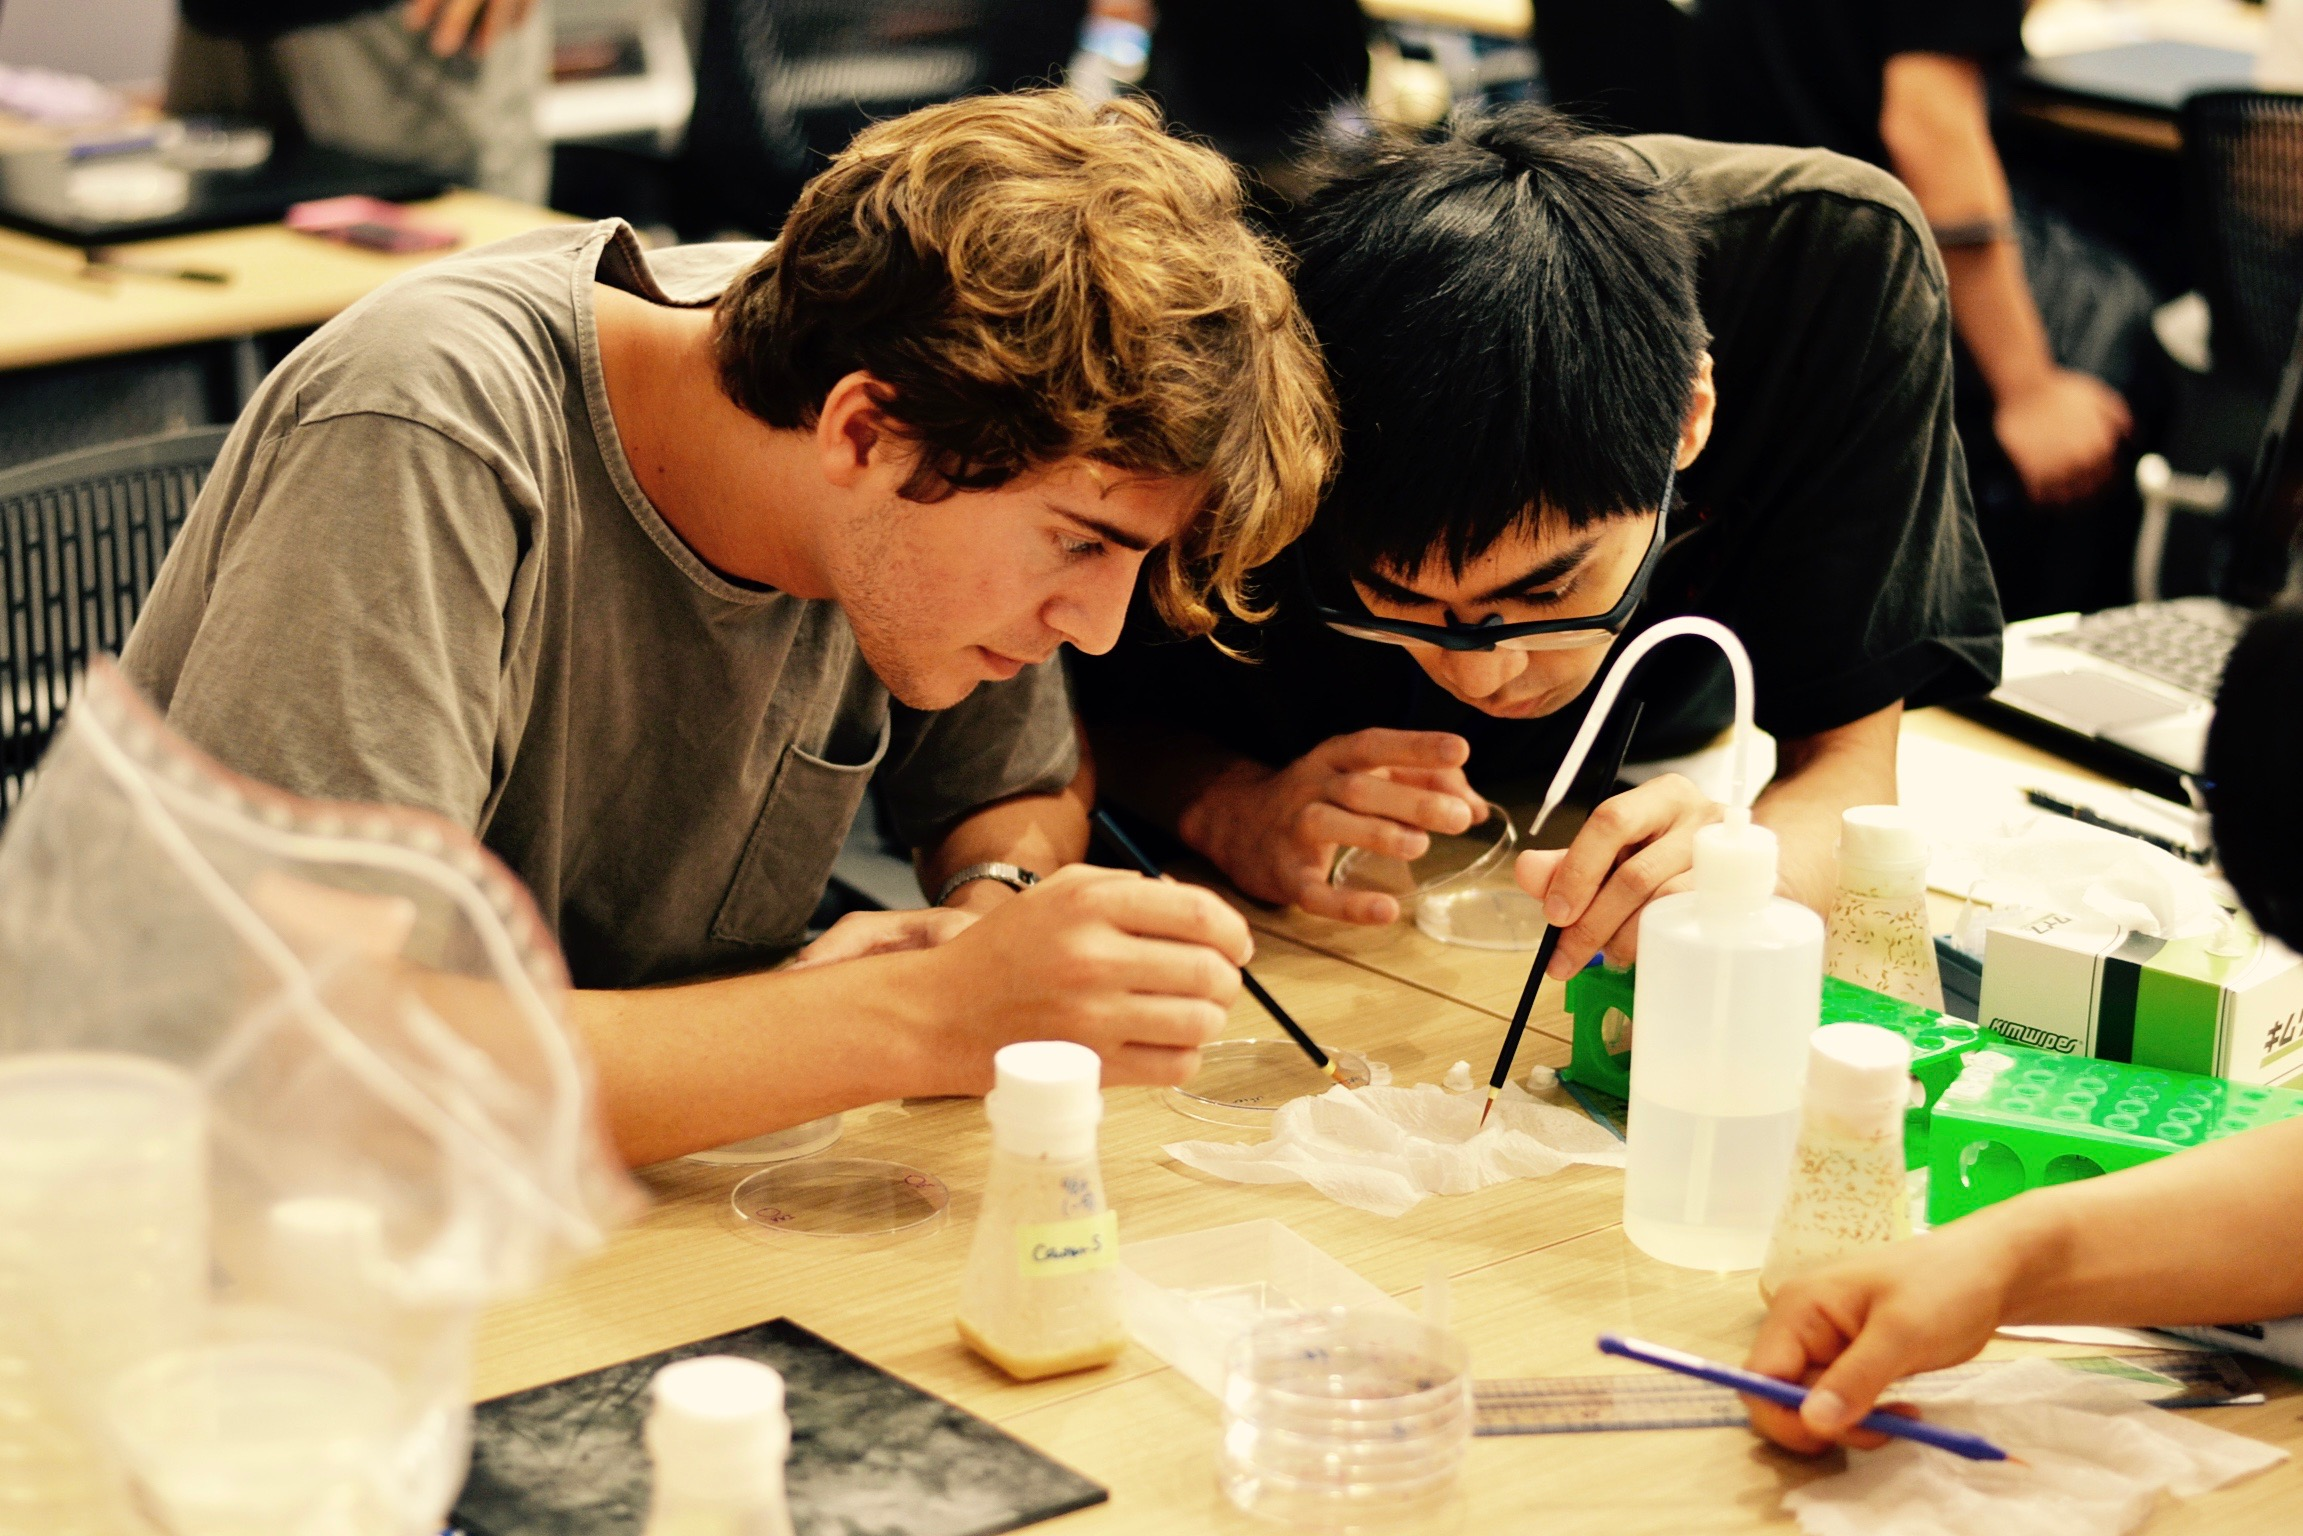
\includegraphics[width=0.4\textwidth]{collaborative_experiment.png}} 
    \subfigure{\includegraphics[width=0.4\textwidth]{presentations_audience.JPG}}\\
    
    \subfigure{\includegraphics[width=0.4\textwidth]{students_on_computers.jpg}}
    \subfigure{\includegraphics[width=0.4\textwidth]{student_presenting.jpg}}  
\end{figure}
\end{frame}



%% TLIA
\begin{frame}
\frametitle{In dieser Vorlesung geht es um\dots}

\begin{center}
    \includegraphics[width=\textwidth]{vlad-tchompalov-nKNrOZ5MXZY-unsplash.jpg}
\end{center}

Wissenschaft, woher sie kommt, und was wir in diesem Modul  vorhaben. 


\end{frame}


%% Learning Objectives
 
\begin{frame}

\frametitle{Nach dieser Vorlesung sollten Sie:}



\begin{block}{Wissen:}
\begin{itemize}
%%%%%
\item
Wissen, was Ihnen im Modul M14 bevorsteht und wie Sie benotet werden

\item
Wichtige historische Entwicklungen benennen
\item 
Grundbegriffe der Erkenntnistheorie benennen und erklären
\item 
Die Grundlagen des kritischen Rationalismus benennen und erklären
\item 
Die Grundlagen des Sozialkonstruktivismus benennen und erklären
\end{itemize}

\end{block}

 

\begin{block}{Können:}
\begin{itemize}
\item
Den historischen und gesellschaftlichen Kontext wissenschaftlicher Forschung erkennen
\item 
Wissenschaftliche Forschung kritisch reflektieren
\end{itemize}
\end{block}

\end{frame}


\begin{frame}

\frametitle{Nach dieser Vorlesung sollten Sie:}

\begin{block}{Fühlen:}

\begin{itemize}
\item
Ihre Rolle als medizinische*r Gelehrte*r reflektieren
\item 
Eine kritische wissenschaftliche Haltung entwickeln
\item 
Sich auf M14 freuen $\heart$
\end{itemize}

\end{block}


\end{frame}


%% Main Body

\section{Willkommen in M14}

%% Warum sind Sie hier?

\begin{frame}{Warum sind Sie hier?}

\begin{itemize}
    \item 
Wollen Sie wissenschaftlich arbeiten?
\item 
Was bedeutet überhaupt  ``wissenschaftliches Arbeiten'' für Sie? 
\item 
Wie wird das in Ihrem späteren Berufsleben relevant sein? 
    
\end{itemize}
    
\end{frame}

%% CanMEDS rollen
\begin{frame}{Ärztliche Rollen: Das CanMEDS Modell}

\begin{center}
    \includegraphics[width=0.6\textwidth]{CanMEDs.jpg}
\end{center}

\tiny{Frank JR, Snell L, Sherbino J, editors. CanMEDS 2015 Physician
Competency Framework. Ottawa: Royal College of Physicians
and Surgeons of Canada; 2015.}


\end{frame}


\begin{frame}{Ärztliche Rollen: Das CanMEDS Modell}


\begin{columns}

\begin{column}{5cm}
\begin{block}{Scholar}
As Scholars, physicians demonstrate a lifelong commitment to excellence in practice through continuous learning and
by teaching others, evaluating evidence, and contributing to scholarship.
\end{block}

\tiny{Richardson D, Oswald A, Chan M-K, Lang ES, Harvey BJ, editors.
Scholar. In: Frank JR, Snell L, Sherbino J, editors. CanMEDS 2015
Physician Competency Framework. Ottawa: Royal College of
Physicians and Surgeons of Canada; 2015}
\end{column}
\begin{column}{5cm}
\begin{center}
    \includegraphics[width=\textwidth]{CanMEDs.jpg}
\end{center}

\end{column}

\end{columns}

\end{frame}

%% Warum bin ich hier?

\begin{frame}{Warum bin ich hier?}

\pause
\begin{columns}[t]

\begin{column}{5cm}
Was Sie denken, dass Ihre Profs im Sommer machen:

\begin{center}
    \includegraphics[width=\textwidth]{chen-mizrach-jL6PTWI7h18-unsplash.jpg}
\end{center}
\end{column}

\pause

\begin{column}{5cm}
Was wir tatsächlich machen: \\[0.8cm]

\begin{center}
    \includegraphics[width=\textwidth]{PhD_movie_screenshot.png}
\end{center}


\end{column}

    
\end{columns}
    
\end{frame}

\begin{frame}{Meine eigene Forschung:}

\centering
\includegraphics[width=0.8\textwidth]{research_triangle_general_blue.png}

\end{frame}


%% Was erwartet uns?
\begin{frame}{Was erwartet uns im Kurs M14?}

7 Vorlesungen, 7 Seminare, schriftliche Abschlussarbeit \\[0.5 cm]

\begin{description}
    \item[Vorlesung 14.1$\,$:] Historische Entwicklung und Grundzüge der Wissenschaftstheorie
\item[Vorlesung 14.2$\,$:] Wissenschaftskulturen und methodische Konsequenzen I: quantitative Forschungsansätze
\item[Vorlesung 14.3$\,$:] Qualitative Forschung
\item[Vorlesung 14.4$\,$:] Formale, ethische und rechtliche Anforderungen an eine wissenschaftliche Arbeit
\item[Vorlesung 14.8$\,$:] Forschungsprozess: Fragestellung generieren
\item[Vorlesung 14.9 und 14.10 $\,$:] Hypothesen formulieren und operationalisieren
\end{description}



\end{frame}


\begin{frame}{Prüfungsleistung für M14}

\begin{block}{Exposé:}

\begin{itemize}
    \item 
    Zusammenfassung der wissenschaftlichen Literatur 
    \item 
    Beschreibung des Aufbaus eines wissenschaftlichen Experiments
    \item 
    Beschreibung und Diskussion der Ergebnisse
    \item 
    Ideen für zusätzliche Forschung
\end{itemize}
    
\end{block}

Gruppenarbeit! \\

Die Bewertungskriterien werden Ihnen online mehrere Wochen vor dem Abgabetermin zur Verfügung gestellt. 

\end{frame}


\begin{frame}{Prüfungsleistung für M14}

\begin{center}
    \includegraphics[width=0.6\textwidth]{Don't_Panic_Badge.jpg}
\end{center}
\end{frame}


\begin{frame}{Prüfungsleistung für M14}
Sie werden in Etappen an die Prüfungsleistung herangeführt und können einen großen Teil der Arbeit innerhalb der Seminare machen. \\[0.5 cm]

\begin{description}
    \item[Seminar 14.5:$\,$] Literaturrecherche in Datenbanken und Bibliotheken
    \item[Seminar 14.6:$\,$] Lesen und Zusammenfassen von Fachliteratur
    \item[Seminar 14.7:$\,$] (Auch) Projektplanung
    \item[Seminar 14.11:$\,$] Festlegung auf Hypothese und Forschungsdesign
    \item[Seminar 14.12:$\,$] Datenerhebung
    \item[Seminar 14.13:$\,$] Datenauswertung
    \item[Seminar 14.14:$\,$] Fertigstellen des Exposés
    
    
\end{description}

\end{frame}

\section{Wissenschaftsgeschichte}

%% Woher wissen wir die Dinge, die wir wissen?

\begin{frame}{Woher wissen Sie die Dinge, die Sie wissen?}
\pause
\begin{itemize}
\item 
Beobachtung/Erfahrung \\
\item 
Experiment \\
\item 
Mündliche Überlieferung \\
\item
Aufgezeichnete Überlieferung \\
\item 
Nachdenken \\

\end{itemize}
\vfill

\textcolor{theme}{Beispiele?}

\end{frame}


\begin{frame}{Woher wissen Sie die Dinge, die Sie wissen?}


\begin{itemize}
    \item 
Beobachtung/Erfahrung \\
\textit{Ich merke, es regnet.}
\item 
Experiment \\
\textit{Ich weiß nicht, wie wasserdicht meine Jacke ist, aber probiere das jetzt aus.}
\item 
Mündliche Überlieferung \\
\textit{Meine Freundin sagt am Telefon, dass es bei ihr in Dresden regnet.}
\item
Aufgezeichnete Überlieferung \\
\textit{Der Wetterbericht sagt, es wird am Nachmittag regnen.}
\item 
Nachdenken \\
\textit{Es wird am Nachmittag regnen und ich habe keinen Schirm dabei. Daher werde ich nass werden.}

\end{itemize}

\end{frame}



%% Wissenschaftsgeschichte
\begin{frame}{Urgeschichte}



\begin{itemize}
    \item 
    Erste Verwendung von Werkzeugen: vor ca. 2.6 Millionen Jahren. 
\item 
Homo sapiens (moderner Mensch) seit ca. 300\,000 Jahren.
\item 
Urgeschichte (=Prähistorie) endet mit der Erfindung der Schrift. 
\item 
Generation und mündliche Überlieferung von Wissen, z.B. für Werkzeugbau, Landwirtschaft (ab Jungsteinzeit), kulturelle und religiöse Traditionen, Behandlung von Krankheiten
\end{itemize}

\end{frame}

\begin{frame}{Urgeschichte}

\begin{center}
    \includegraphics[width=0.8\textwidth]{Crane-trepanation-img_0507.jpg}
\end{center}

Trepanierter Schädel aus der Jungsteinzeit (3\,500 Jahre v.u.Z.)

\end{frame}

\begin{frame}{Schriftliche Kulturen}

Erfindung der Schrift ca. 4 Mal in der Menschheitsgeschichte vor 2\,000-5\,400 Jahren (Mesopotamien, Ägypten, China, Mittelamerika) \\
\vfill

\centering
\includegraphics[width=0.5\textwidth]{Writing_system_survey.png}

\end{frame}


\begin{frame}{Schriftliche Kulturen}

\begin{columns}[c]
    \begin{column}{5cm}
\begin{itemize}
    \item 
    Schrift erlaubt Aufzeichnung und weite Transmission von Wissen
    \item 
    Fortschritte z.B. in Medizin, Technologie, Mathematik, Astronomie, Philosophie
    \item 
    Internationaler Wissenstransfer entlang von Handelsrouten (z.B. indischer Subkontinent - arabische Halbinsel - römisches Reich)
\end{itemize}
        
    \end{column}

\begin{column}{5cm}
\includegraphics[width=\textwidth]{Papyrus_Ebers.png}
Papyrus Ebers, ca. 1550 v.u.Z. 

\end{column}
    
\end{columns}

\end{frame}



\begin{frame}{(Europäisches) Mittelalter}

\begin{itemize}
    \item Rezeption und Übersetzung von griechischen und arabischen Texten
    \item Bewahrung und Weitergabe von Wissen in Klöstern, daher oft religiöser Einfluss
    
\end{itemize}

\begin{columns}[c]

\begin{column}{5cm}
\begin{itemize}
    \item Gründung von Universitäten (z.B. Bologna, 1088)
    \item 
    Universitäre Ausbildung für Recht, Medizin, Theologie
    \item 
    Fokus der Wissenschaft auf Deduktion (Ableitung von Wissen aus Theorien), der antiken griechischen Tradition folgend

\end{itemize}
    
\end{column}



    \begin{column}{5cm}
\includegraphics[width=\textwidth]{Oxfordceremony.jpg}    
\end{column}

\end{columns}


\end{frame}

\begin{frame}{Induktion vs Deduktion}

\centering

\includegraphics[width=\textwidth]{Induktion-Deduktion.svg.png}



\end{frame}

\begin{frame}{Naturwissenschaftliche Revolution in Europa}

\begin{itemize}
    \item 
    Frühe Neuzeit (16./17. Jahrhundert)
    \item 
    Relativ neue Entwicklungen: Buchdruck, religiöse Spaltungen, Aufklärung, Erkundung und Kolonisierung anderer Kontinente
    \item 
    Stärkere Hinwendung zu Erkenntnisgewinnung durch Experiment (Induktion)
    \item 
    Bau von wissenschaftlichen Instrumenten: Mikroskope, Teleskope, Laborgeräte, \dots
    \item 
    Etwas später: Institutionalisierung und Professionalisierung von Wissenschaft. \textcolor{theme}{Was bedeutet das? Wer war dabei? Wer nicht?}
    \end{itemize}
    
\end{frame}






\begin{frame}{Aktuell}

Wie verändert sich die Wissenschaft im Moment? Was tragen neue Technologien wie leistungsstarke vernetzte Computer, künstliche Intelligenz und soziale Medien dazu bei?

\centering


\includegraphics[width=0.8\textwidth]{markus-spiske-iar-afB0QQw-unsplash.jpg}
    
\end{frame}


\section{Wissenschaftstheorie}

%% wissenschaftslehre, kritischer Rationalismus
\begin{frame}{Einige Definitionen}

\begin{description} 
    \item[Erkenntnistheorie/Epistemologie:] Gebiet der Philosophie, das sich damit befasst, wie Wissen zustande kommt
    \item[Wissenschaftstheorie:] Gebiet der Philosophie, das untersucht, wie wissenschaftliche Erkenntnisse gewonnen werden (oder werden sollen)
    \item[Science and Technology Studies (STS):] Interdisziplinäres Feld. Untersucht, wie wissenschaftliche Erkenntnisgewinnung im Kontext (z.B. gesellschaftlich, politisch, historisch) vor sich geht


\end{description}
    
\end{frame}

\begin{frame}{Fragen der Wissenschaftstheorie (Beispiele)}

\begin{itemize}
    \item Was ist das Ziel von Wissenschaft?
    \item Mit welchen Methoden können wissenschaftliche Erkenntnisse gewonnen werden?
    \item Mit welchen Methoden werden wissenschaftliche Erkenntnisse tatsächlich gewonnen?
    \item Was ist eine gute wissenschaftliche Theorie?
    \item Was braucht es, um eine Theorie zu bestätigen oder zu widerlegen?
    \item Welche ethischen Verpflichtungen haben Wissenschafter*innen?
    \item 
    In welchem gesellschaftlichen Kontext passiert Wissenschaft?
\end{itemize}

Viele Modelle und Theorien existieren, wir betrachten heute nur kurz zwei Beispiele

\end{frame}

\begin{frame}{Beispiel: Kritischer Rationalismus}

Kurze Erinnerung:

\centering

\includegraphics[width=\textwidth]{Induktion-Deduktion.svg.png}



\end{frame}


\begin{frame}{Beispiel: Kritischer Rationalismus}

\begin{columns}[c]

\begin{column}{5cm}

\begin{itemize}
    \item 
Induktion geht gar nicht. \textcolor{theme}{Warum?}
\item 
Theorien sind grundsätzlich nicht beweisbar, müssen aber falsifizierbar sein.
\item 
Theorien können systematisch geprüft werden (``Trial and Error''). 
\item 
Falsifizierte Theorien müssen über den Haufen geworfen werden.

    
\end{itemize}

    
\end{column}

\begin{column}{5cm}

\includegraphics[width=\textwidth]{Karl_Popper.jpg}


Sir Karl Popper (1902-1994)
    
\end{column}



    
\end{columns}

\end{frame}


\begin{frame}{Beispiel: Sozialkonstruktivismus}
    
\begin{columns}[c]


\begin{column}{5cm}

\includegraphics[width=\textwidth]{Knorr_Cetina_Karen.jpg}


Karin Knorr-Cetina (*1944)
    
\end{column}




\begin{column}{6cm}
\begin{itemize}
\item 
Basierend auf ethnologischen Beobachtungen in Forschungslaboren
    \item
"Klassischer" Weg von Hypothese zu Experiment stimmt in der Praxis nicht
    \item
    Wissenschaftliche Produktion unterliegt sozialen Regeln
    \item 
    ``Labor-Opportunismus'': Was von wem wie erforscht wird, hängt von den Bedingungen ab (z.B. Laborausstattung, strategische Überlegungen, \dots) 
    
\end{itemize}

    
\end{column}


    
\end{columns}

\end{frame}


\begin{frame}{Was stimmt denn jetzt?}

\centering

\includegraphics[width=0.8\textwidth]{jon-tyson-hhq1Lxtuwd8-unsplash.jpg}

\end{frame}

\begin{frame}{Was stimmt denn jetzt?}

Das können wir nicht innerhalb dieser Vorlesung entscheiden. Erkenntnistheoretische Modelle sollen uns beim Nachdenken helfen. \\[0.5] 

Mir ist wichtig, dass Sie (oft und Ihr ganzes Leben lang!) über Wissenschaft nachdenken, z.B.:

\begin{itemize}
    \item 
    Was sind noch offene Fragen? Was müsste gemacht werden, um sie zu klären?
    \item 
    In welchem Kontext findet Wissenschaft statt? Wer hat welche Gründe? Wer darf teilhaben? Wer ist ausgeschlossen?
    \item 
    Was ist mein Kontext? Wie macht sich meine Subjektivität bemerkbar? Welchen Fehlern sitze ich möglicherweise auf? 
    \item 
    Was sind die möglichen ethischen Folgen meiner Forschung? 
\end{itemize}


\end{frame}

%% Fallen


%% Lesen
\begin{frame}

\frametitle{Literaturempfehlung}

\begin{itemize}
    \item 
    Das CanMEDS Framework zu ärztlichen Rollen (auf Englisch):  \\
    Frank JR, Snell L, Sherbino J, editors. CanMEDS 2015 Physician
Competency Framework. Ottawa: Royal College of Physicians
and Surgeons of Canada; 2015.  \url{https://www.royalcollege.ca/en/standards-and-accreditation/canmeds.html}

\end{itemize}

Falls Sie etwas mehr Zeit haben:

\begin{itemize}

\item 
Karl Popper. Logik der Forschung. Zur Erkenntnistheorie der modernen Naturwissenschaft (1935). Zahlreiche Neuauflagen existieren.

\item 
Karin Knorr-Cetina. Die Fabrikation von Erkenntnis. Zur Anthropologie der Naturwissenschaft, Suhrkamp, Frankfurt am Main (1984), erweiterte Neuauflage 2002.

\end{itemize}


\end{frame}



%% Review




\begin{frame}

\frametitle{Jetzt* sollten Sie:}



\begin{block}{Wissen:}
\begin{itemize}
%%%%%
\item
Wissen, was Ihnen im Modul M14 bevorsteht und wie Sie benotet werden

\item
Wichtige historische Entwicklungen benennen
\item 
Grundbegriffe der Erkenntnistheorie benennen und erklären
\item 
Die Grundlagen des kritischen Rationalismus benennen und erklären
\item 
Die Grundlagen des Sozialkonstruktivismus benennen und erklären
\end{itemize}

\end{block}

 

\begin{block}{Können:}
\begin{itemize}
\item
Den historischen und gesellschaftlichen Kontext wissenschaftlicher Forschung erkennen
\item 
Wissenschaftliche Forschung kritisch reflektieren
\end{itemize}
\end{block}

\end{frame}


\begin{frame}

\frametitle{Jetzt* sollten Sie:}

\begin{block}{Fühlen:}

\begin{itemize}
\item
Ihre Rolle als medizinische*r Gelehrte*r reflektieren
\item 
Eine kritische wissenschaftliche Haltung entwickeln
\item 
Sich auf M14 freuen $\heart$
\end{itemize}

\end{block}


\end{frame}





%% Feedbackhinweisblock

\begin{frame}
\frametitle{Danke für Ihr Feedback!}
\begin{center}
\includegraphics[width=0.6\textwidth]{feedback_QR.png}
\end{center}

\end{frame}





%% Bildnachweis
\begin{frame}
\frametitle{Bildnachweis}

\vfill

\begin{tiny}
\begin{itemize}
\item 
CanMEDS Rollen. Eigenes Werk. CC-BY-SA 4.0, 2024. 

\item 
Convocation (Abschlussfeier) in Oxford. Public Domain, \url{https://commons.wikimedia.org/w/index.php?curid=532844}

\item 
Don't Panic. Jim Linwood, CC BY 2.0 \url{https://creativecommons.org/licenses/by/2.0}, via Wikimedia Commons

\item 
Forschung im Stefan Lab. Eigenes Werk. CC-BY-SA 4.0, 2017.

\item 
Fragezeichen. Photo by \href{https://unsplash.com/@jontyson?utm_content=creditCopyText&utm_medium=referral&utm_source=unsplash}{Jon Tyson} on \href{https://unsplash.com/photos/white-markee-light-hhq1Lxtuwd8?utm_content=creditCopyText&utm_medium=referral&utm_source=unsplash}{Unsplash}
  

\item 
Frau am Strand. Photo by \href{https://unsplash.com/@chenhanozel?utm_content=creditCopyText&utm_medium=referral&utm_source=unsplash}{Chen Mizrach} on \href{https://unsplash.com/photos/woman-sits-on-brown-wooden-beach-chair-jL6PTWI7h18?utm_content=creditCopyText&utm_medium=referral&utm_source=unsplash}{Unsplash}
%% all lectures

\item 
Induction und Deduktion WissensDürster, Public domain, via Wikimedia Commons \url{https://commons.wikimedia.org/wiki/File:Induktion-Deduktion.svg}
\item 
Karin Knorr-Cetina. University of Chicago, Division of Social Sciences. \url{https://socialsciences.uchicago.edu/directory/Karin-Knorr-Cetina}

\item
Logo der MSB. MSB Medical School Berlin, Public Domain, via Wikimedia Commons
\item 
March for Science. Photo by \href{https://unsplash.com/@tchompalov?utm_content=creditCopyText&utm_medium=referral&utm_source=unsplash}{Vlad Tchompalov} on \href{https://unsplash.com/photos/group-of-people-with-signages-nKNrOZ5MXZY?utm_content=creditCopyText&utm_medium=referral&utm_source=unsplash}{Unsplash}
\item 
Matrix-ähnliches Bild, um die digitale Revoultion zu illustrieren. Photo by \href{https://unsplash.com/@markusspiske?utm_content=creditCopyText&utm_medium=referral&utm_source=unsplash}{Markus Spiske} on \href{https://unsplash.com/photos/matrix-movie-still-iar-afB0QQw?utm_content=creditCopyText&utm_medium=referral&utm_source=unsplash}{Unsplash}
  

\item 
Papyrus Ebers. By Unknown scribe - \url{https://www.nlm.nih.gov/hmd/breath/breath_exhibit/MindBodySpirit/IIBa18.html}, Public Domain, \url{https://commons.wikimedia.org/w/index.php?curid=1606171}


\end{itemize}

\end{tiny}
\end{frame}

\begin{frame}
\frametitle{Bildnachweis}

\vfill

\begin{tiny}
\begin{itemize}


  

\item 
Schriftsysteme. By Ian Remsen - Own work, CC0, \url{https://commons.wikimedia.org/w/index.php?curid=151455271}

\item 
Sir Karl Popper. Von LSE library - \url{https://www.flickr.com/photos/lselibrary/3833724834/in/set-72157623156680255/}, No restrictions, \url{https://commons.wikimedia.org/w/index.php?curid=9694262}

  
\item 
Studierende beim gemeinsamen Experimentieren, bei der Arbeit an ihren Computern und beim Präsentieren von Daten. Yuuki Guzman und Agoston Tyll, Okinawa Institute of Science and Technology, 2015 und 2016. 

\item 
Trepanierter Schädel. Rama, CC BY-SA 3.0 FR \url{https://creativecommons.org/licenses/by-sa/3.0/fr/deed.en}, via Wikimedia Commons

\item 
Zwei Forschende in Labormäntel. Screenshot aus Cham, J. (2011) Piled Higher and Deeper. 

\end{itemize}

\end{tiny}
\end{frame}


\end{document}
